\chapter{지평선, 상태방정식, 진공 에너지}

\section{선호 기준계, 초광속 후퇴, 지평선}

우주 마이크로파 배경복사는 실제로 특별한 기준계를 정해 준다. 이 복사가 등방적으로 보이는 기준계에서는 가까운 은하들도 평균적으로 정지해 있다. 우리가 배경복사에 대해 움직이면 진행 방향의 광자는 도플러 효과로 에너지가 높아지고, 반대 방향의 광자는 에너지가 낮아진다. 선호 기준계는 마이크로파 배경복사가 등방적으로 보이는 기준계이며, 평균적으로 국소 은하들이 정지해 있는 기준계이기도 하다.

\begin{classroomqa}
\lecturetimestamp{00:00:25}
\audiencequestion{우주 복사의 겉보기 파장은 관측자의 운동에 따라 달라지나요? 그렇다면 선호 기준계가 있다는 뜻인가요?}
\lecturerresponse{그렇습니다. 마이크로파 배경복사에 대해 움직이면 도플러 비등방성이 생기므로 우주론적 선호 기준계가 있습니다. 마이크로파 배경복사가 등방적으로 보이는 기준계가 바로 그것입니다. 이 기준계는 평균적으로 국소 은하들이 정지해 있는 기준계이기도 합니다.}
\end{classroomqa}

두 번째 질문은 후퇴 속도에 관한 것이다. 허블 법칙에 따르면 충분히 먼 은하들은 다음과 같은 속도로 서로 멀어진다.
\begin{equation}
v = H d .
\end{equation}
\(d\)가 충분히 크면 이 후퇴 속도는 빛의 속도를 넘는다. 이것은 상대성이론과 모순되지 않는다. 금지되는 것은 국소적인 상황, 즉 한 물체가 우리 바로 앞에서 다른 물체를 빛보다 빠르게 앞질러 가는 일이기 때문이다. 먼 은하들에 관한 진술은 서로 멀리 떨어진 장소들 사이의 기하에 관한 것이다.

\begin{classroomqa}
\lecturetimestamp{00:04:48}
\audiencequestion{두 은하 사이의 상대 속도가 \(c\)보다 클 수 있나요?}
\lecturerresponse{그렇습니다. 두 은하가 충분히 멀리 떨어져 있다면 가능합니다. 허블 후퇴 속도가 빛의 속도를 넘더라도 국소적 상대성이론을 위반하지 않습니다. 후퇴 속도가 \(c\)에 이르는 곳이 지평선입니다.}
\end{classroomqa}

후퇴 속도가 빛의 속도에 이르면 우리를 향해 보낸 신호는 더 이상 순수하게 우리 쪽으로 다가오지 못한다. 광선은 국소적으로 한계 속도로 움직이지만, 광선이 따라잡아야 할 거리가 너무 빠르게 늘어나기 때문이다.

\begin{classroomqa}
\lecturetimestamp{00:07:03}
\audiencequestion{반대 방향으로 보낸 광선은 그래도 우리 쪽으로 이동하지 않나요?}
\lecturerresponse{국소적으로는 그렇지만, 공간이 광선이 따라잡을 수 있는 속도보다 더 빠르게 팽창합니다. 광선은 가까운 점들에 대해 한계 속도로 움직이는 한편, 우리까지의 전체 거리는 계속 늘어납니다.}
\end{classroomqa}

\section{팽창하는 계량과 선의 비유}

1차원 그림을 생각하면 이해하기 쉽다. 원자들로 이루어진 선을 상상해 보자. 보통의 물질로 된 선을 잡아당기면 결국 끊어진다. 이제 그림을 조금 바꿔 보자. 이웃한 원자들이 너무 멀어질 때마다 그 사이에 원자를 하나씩 넣는다. 선은 계속 늘어나지만 국소적인 성질은 희박해지지 않는다.

\begin{figure}
\centering
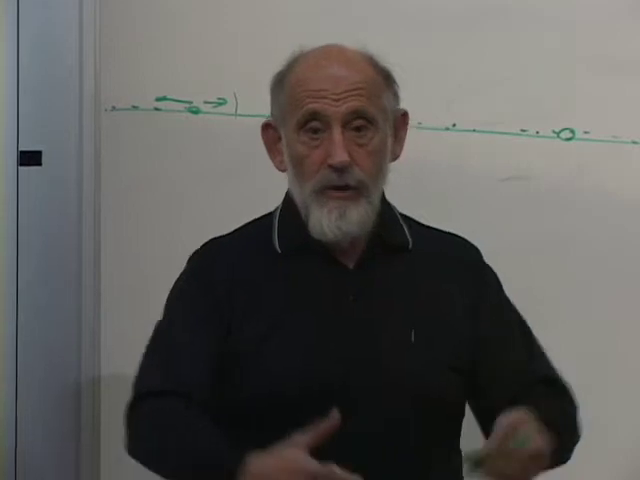
\includegraphics[width=0.60\textwidth]{lecture_04_figure_02.png}
\caption{팽창하는 계량을 나타내는 1차원 선의 비유.}
\end{figure}

이 그림에서도 국소적인 신호의 한계 속도는 여전히 존재한다. 보통의 선에서 소리가 한계 속도를 갖는 것과 같다. 규칙은 국소적이다. 교란은 가까운 점들에 대해 그 속도를 넘어설 수 없다. 그래도 선이 충분히 길고 새로운 점들이 충분히 빠르게 삽입되면, 충분히 멀리 떨어진 부분들은 신호가 끝내 돌아올 수 없을 만큼 빠르게 멀어진다.

따라서 특수상대론의 속도 합성 법칙은 이야기의 일부일 뿐이다. 이 법칙은 관측자들이 같은 지점에서 서로 지나칠 때 국소적으로 적용된다. 팽창하는 기하에서 멀리 떨어진 은하들을 다룰 때는 적절한 도구가 아니다.

\begin{classroomqa}
\lecturetimestamp{00:09:42}
\audiencequestion{이 상황에서도 보통의 상대론적 속도 합성 법칙이 성립하나요?}
\lecturerresponse{국소적으로, 한 지점에서는 그렇습니다. 관측자들이 차례로 서로를 지나친다면 보통의 특수상대론적 법칙이 적용됩니다. 하지만 \(c\)보다 빠른, 멀리 떨어진 천체들의 후퇴를 설명하는 데는 적절하지 않습니다. 그런 경우에는 팽창하는 공간의 기하를 살펴봐야 합니다.}
\end{classroomqa}

이 그림은 적색편이도 간단히 설명해 준다. 선 위에 파동을 그려 보자. 선이 팽창하면 파장도 함께 늘어난다. 팽창하는 기하에서는 이것이 단지 이해를 돕기 위한 비유에 그치지 않는다. 팽창하는 시공간의 파동 방정식은 실제로 늘어난 파장을 예측한다.

\begin{classroomqa}
\lecturetimestamp{00:14:42}
\audiencequestion{파동이 우주와 함께 늘어난다는 설명은 이론적인가요, 관측에 근거한 것인가요, 아니면 둘 다인가요?}
\lecturerresponse{팽창하는 시공간에서 파동이 전파될 때 이론적으로 따라 나오는 결과이며, 천문 관측으로도 뒷받침됩니다.}
\end{classroomqa}

이 그림은 고무줄과 다르다. 고무줄은 늘어나면 가늘어지고, 그런 매질 속에 사는 관측자는 국소적 성질이 변하는 것을 보게 된다. 여기서는 전역적인 거리 척도만 커질 뿐 국소적인 성질은 그대로 유지된다.

\section{최종 산란과 관측 가능한 우주}

지평선은 후퇴 속도가 빛의 속도에 이르는 곳이다. 최종 산란면은 그보다 약간 안쪽에 있다. 지평선에서 방출된 신호의 파장은 한없이 늘어나지만, 최종 산란 복사의 적색편이는 매우 크더라도 유한하다.

\begin{classroomqa}
\lecturetimestamp{00:17:53}
\audiencequestion{초광속 후퇴, 최종 산란면, 관측 가능한 우주는 어떤 관계인가요?}
\lecturerresponse{지평선은 후퇴 속도가 빛의 속도에 이르는 곳입니다. 최종 산란면은 적색편이가 엄청나게 크지만 유한하기 때문에 그보다 약간 안쪽에 있습니다. 실용적인 의미에서 최종 산란면은 관측 가능한 우주의 경계를 나타냅니다.}
\end{classroomqa}

최종 산란 복사의 적색편이는 대략 \(10^3\)배이다. 이 정도로도 최종 산란면은 여러 목적에서 지평선에 매우 가깝다. 관측 가능한 우주는 빛이 우리에게 도달할 수 있는 우주의 일부다.

후기에는 팽창이 진공 에너지 지배 영역에 가까워진다. 그러면 허블 매개변수는 일정한 값에 가까워지고, 지평선의 크기는 고정된 값에 가까워지며, 은하와 마이크로파 복사는 모두 점차 시야에서 사라진다.

\begin{classroomqa}
\lecturetimestamp{00:22:43}
\audiencequestion{\(H\)는 시간에 따라 변하는데, 지평선 거리는 변하나요? 마이크로파 배경복사는 결국 사라지나요?}
\lecturerresponse{후기에는 \(H\)가 일정한 값에 가까워지므로 지평선은 고정된 거리에 가까워집니다. 마이크로파 배경복사는 계속 늘어나고 식으면서 희미해집니다. 먼 은하들도 지평선을 지나 시야에서 사라집니다.}
\end{classroomqa}

이미 중력적으로 묶여 있는 구조만 시야에 남는다. 태양계는 흩어지지 않고 은하도 흩어지지 않지만, 큰 규모의 우주는 고립된 섬이 된다.

\section{기본 팽창 방정식과 세 성분}

이제 기본 팽창 방정식은 다음과 같다.
\begin{equation}
\left(\frac{\dot a}{a}\right)^2 = \frac{8\pi G}{3}\rho ,
\qquad c=1 .
\end{equation}
여기서 \(a(t)\)는 척도인자이고, \(\rho\)는 전체 에너지 밀도다.

\begin{figure}
\centering
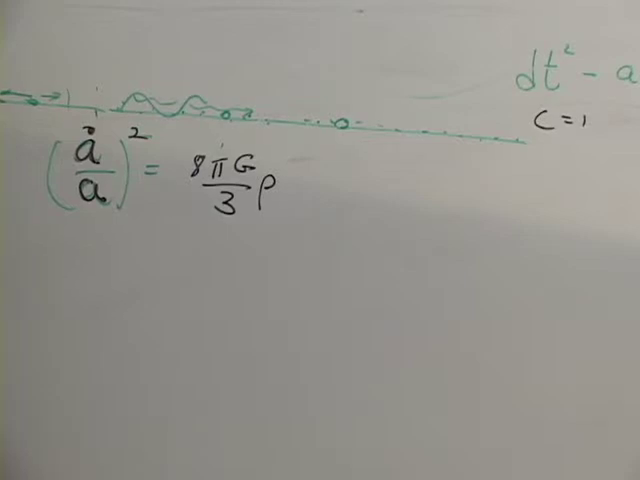
\includegraphics[width=0.74\textwidth]{lecture_04_figure_03.png}
\caption{기본 팽창 방정식과 1차원 선의 비유.}
\end{figure}

동역학적으로 중요한 성분은 세 가지다.

물질의 경우,
\begin{equation}
\rho=\frac{\text{const.}}{a^3},
\qquad
a(t)\sim t^{2/3}.
\end{equation}
이는 질량을 가진 물체들이 전체 팽창을 따라 움직이며 공변 기준계에서는 사실상 정지해 있는 경우다.

복사의 경우,
\begin{equation}
\rho=\frac{\text{const.}}{a^4},
\qquad
a(t)\sim t^{1/2}.
\end{equation}
\(a\)의 추가 거듭제곱은 우주가 팽창하면서 각 광자의 파장이 늘어나는 데서 비롯된다.

또한 다음 성분이 있다.
\begin{equation}
\rho_0=\text{constant},
\end{equation}
진공 에너지이며, 암흑 에너지라고도 하고 통상적인 수치 계수를 제외하면 우주 상수라고도 한다. 이 성분은 전혀 희석되지 않는다.

다음 단계는 에너지 밀도와 압력을 연결하는 것이다.

\section{복사 압력과 차가운 물질}

복사부터 살펴보자. 길이 \(L\)인 선분 하나만 있는 1차원 상자를 생각하자. 그 안에는 광자들이 앞뒤로 튕겨 다닌다. 1차원에서는 힘과 압력이 사실상 같은 양이다.

운동량 크기가 \(p\)인 광자를 생각하자. 광자가 벽에 반사될 때 운동량 변화는 다음과 같다.
\begin{equation}
\Delta p = 2p.
\end{equation}
같은 벽에 연속해서 충돌할 때까지의 시간은
\begin{equation}
\Delta t = \frac{2L}{c}.
\end{equation}
따라서 벽이 받는 평균 힘은
\begin{equation}
F=\frac{\Delta p}{\Delta t}=\frac{pc}{L}.
\end{equation}
광자의 경우,
\begin{equation}
E=pc,
\end{equation}
이므로
\begin{equation}
F=\frac{E}{L}.
\end{equation}
에너지를 길이로 나눈 값은 1차원 에너지 밀도다. 이 1차원 사례에서는
\begin{equation}
P=\rho .
\end{equation}

광자가 많더라도 평균을 취하면 같은 관계가 성립한다. 전체 힘은 단위 길이당 전체 에너지와 같다.

이제 3차원으로 가 보자. 모든 광자가 한 축을 따라서만 움직인다면 한 쌍의 면에는 압력을 가하지만 나머지 면에는 압력을 가하지 않는다. 일부러 틀린 가정이지만, 무엇을 바로잡아야 하는지는 바로 드러난다. 등방적인 복사에서는 운동량이 모든 방향으로 분포한다. 평균적으로 에너지 밀도의 3분의 1이 각 압력 성분에 기여한다. 따라서
\begin{equation}
P=\frac{\rho}{3}.
\end{equation}

차가운 물질의 경우에는 답이 다르다. 우주의 흐름을 따라 움직이는 작은 영역인 공변 상자를 생각하자. 안에 있는 입자들은 에너지를 갖고 있지만, 상자에 대해 정지해 있다면 벽에 부딪치지 않는다. 따라서 압력은
\begin{equation}
P=0.
\end{equation}

\begin{figure}
\centering
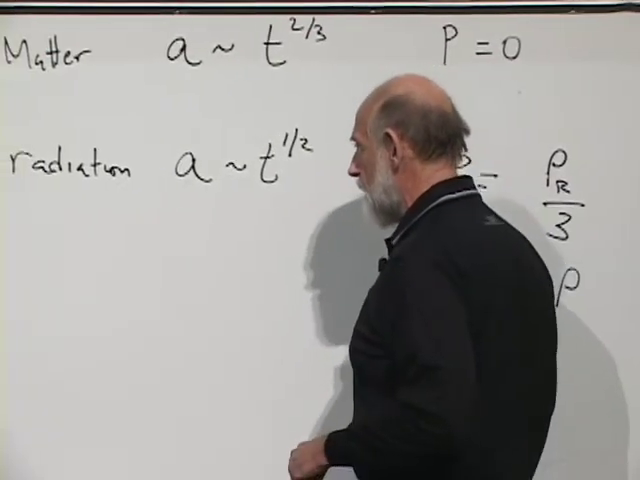
\includegraphics[width=0.74\textwidth]{lecture_04_figure_04.png}
\caption{물질과 복사: \(a\sim t^{2/3}\), \(P=0\), 그리고 \(a\sim t^{1/2}\), \(P=\rho/3\).}
\end{figure}

칠판의 요약은 다음과 같다.
\begin{align}
\text{matter:}\qquad & a(t)\sim t^{2/3}, \qquad P=0,\\
\text{radiation:}\qquad & a(t)\sim t^{1/2}, \qquad P=\frac{\rho}{3}.
\end{align}

\begin{classroomqa}
\lecturetimestamp{00:54:27}
\audiencequestion{팽창하는 우주에서 입자들이 실제로 서로 멀어지고 있지 않나요?}
\lecturerresponse{그렇습니다. 하지만 압력에 관한 논증은 무한소 크기의 공변 상자에 적용됩니다. 그 국소적인 규모에서는 열역학적 추론이 여전히 성립합니다.}
\end{classroomqa}

\section{상태방정식}

압력은 에너지 밀도에 비례한다고 둔다.
\begin{equation}
P=w\rho .
\end{equation}
칠판에서는 같은 매개변수를 \(\omega\)로 쓴다. 기본적인 두 경우는 다음과 같다.
\begin{equation}
w=0 \quad \text{for cold matter},
\qquad
w=\frac{1}{3} \quad \text{for radiation}.
\end{equation}

그 사이의 값도 가능하다. \(0\)와 \(1/3\) 사이의 값은 완전히 차갑지도 완전히 상대론적이지도 않은 물질을 나타낸다. 여기서 언급하는 예는 따뜻한 암흑 물질이다.

\begin{figure}
\centering
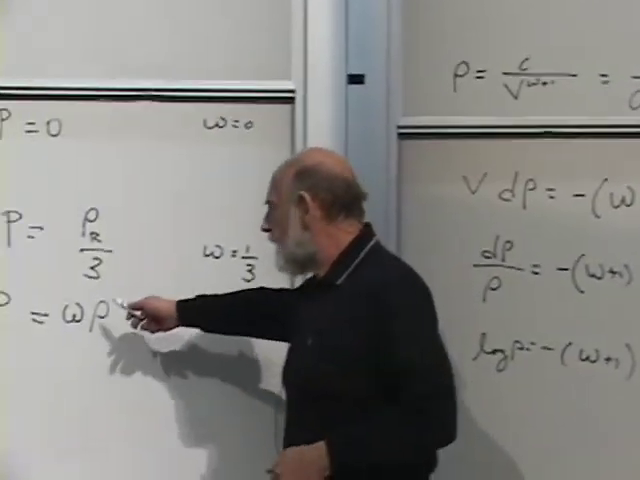
\includegraphics[width=0.74\textwidth]{lecture_04_figure_05.png}
\caption{상태방정식 \(P=\omega\rho\)과 밀도 스케일링 논증.}
\end{figure}

다음 질문은 \(w\)가 \(a\)에 따른 \(\rho\)의 변화를 결정하는가이다. 답은 열역학 항등식에서 나온다.

부피가 \(V\)인 상자를 생각하자. 내용물이 압력 \(P\)을 가할 때 상자가 \(dV\)만큼 팽창하면 벽에 한 일은 다음과 같다.
\begin{equation}
dE=-P\,dV.
\end{equation}
이제 에너지를 다음과 같이 쓰자.
\begin{equation}
E=\rho V.
\end{equation}
그 미분은
\begin{equation}
dE=\rho\,dV+V\,d\rho .
\end{equation}
두 식을 같게 놓으면
\begin{equation}
\rho\,dV+V\,d\rho=-P\,dV,
\end{equation}
또는
\begin{equation}
V\,d\rho=-(\rho+P)\,dV.
\end{equation}
\(P=w\rho\)를 사용하면,
\begin{equation}
V\,d\rho=-(1+w)\rho\,dV.
\end{equation}
\(\rho V\)로 나누면,
\begin{equation}
\frac{d\rho}{\rho}=-(1+w)\frac{dV}{V}.
\end{equation}
적분하면,
\begin{equation}
\rho \propto V^{-(1+w)}.
\end{equation}
공변 우주론적 상자에서는
\begin{equation}
V\propto a^3,
\end{equation}
따라서
\begin{equation}
\rho \propto a^{-3(1+w)}.
\end{equation}

앞서 본 경우들은 곧바로 얻어진다.
\begin{align}
w=0 &\Longrightarrow \rho \propto a^{-3},\\
w=\frac{1}{3} &\Longrightarrow \rho \propto a^{-4}.
\end{align}

이 때문에 \(w\)가 중요하다. \(\rho(a)\)를 알면 이를 프리드만 방정식에 대입할 수 있다. 그런 다음 거듭제곱 법칙 \(a\sim t^\alpha\)를 가정해 보고, 해당 상태방정식에서 우주가 어떻게 팽창하는지 구한다.

\section{진공 에너지와 음의 압력}

한 가지 특별한 경우는 다르게 거동한다.
\begin{equation}
w=-1.
\end{equation}
그러면
\begin{equation}
1+w=0,
\end{equation}
따라서 지수가 0이 되고,
\begin{equation}
\rho=\rho_0=\text{constant}.
\end{equation}
이에 해당하는 압력은
\begin{equation}
P=-\rho .
\end{equation}

음의 압력 자체가 신비로운 것은 아니다. 양의 압력은 상자의 벽을 바깥쪽으로 민다. 음의 압력은 안쪽으로 당긴다. 즉 장력이다. 늘어난 고무줄이 일상적인 예다. 고무줄은 양의 에너지를 저장하지만 양 끝을 서로 끌어당긴다.

일정한 밀도 \(\rho_0\)를 프리드만 방정식에 대입하면,
\begin{equation}
\left(\frac{\dot a}{a}\right)^2=\frac{8\pi G}{3}\rho_0.
\end{equation}
우변은 상수이므로
\begin{equation}
\frac{\dot a}{a}=\sqrt{\frac{8\pi G}{3}\rho_0}.
\end{equation}
허블 매개변수가 실제로 일정한 특별한 경우다. 방정식은 다음과 같이 쓸 수 있고,
\begin{equation}
\dot a=\sqrt{\frac{8\pi G}{3}\rho_0}\,a,
\end{equation}
해는 다음과 같다.
\begin{equation}
a(t)\propto \exp\!\left(\sqrt{\frac{8\pi G}{3}\rho_0}\,t\right).
\end{equation}

이는 지수 팽창이다. 관련된 시간 척도는 배가 시간이 아니라 \(e\)배 시간이므로, 여기서 사용하는 대략적인 추정에 따르면 우주의 나이와 비슷한 규모다. 진공 에너지와 우주 상수는 역사적인 수치 관례를 제외하면 같은 물리적 성분이다.

\begin{classroomqa}
\lecturetimestamp{01:27:16}
\audiencequestion{진공 에너지가 지수 팽창을 일으킨다면 결국 모든 것이 찢겨 나가지 않나요?}
\lecturerresponse{반드시 그렇지는 않습니다. 묶인 계는 팽창에 저항할 수 있습니다. 은하, 태양계, 원자는 반드시 찢겨 나가는 것이 아닙니다. 반면 충분히 크고 희박한 구조는 팽창에 참여해 결국 서로 멀어집니다.}
\end{classroomqa}

\begin{classroomqa}
\lecturetimestamp{01:31:43}
\audiencequestion{프리드만 방정식의 제곱근을 취할 때 나오는 음의 부호에도 흥미로운 의미가 있나요?}
\lecturerresponse{그렇습니다. 제곱근을 취하면 두 가지 해가 나옵니다. 하나는 팽창 해이고, 다른 하나는 시간 반전된 수축 해입니다. 방정식 자체는 둘 다 허용합니다.}
\end{classroomqa}

\section{세 시대와 관측된 팽창 역사}

세 성분이 모두 존재하며, 각각 다음과 같이 스케일링한다.
\begin{equation}
\begin{aligned}
\rho_{\text{radiation}}&\propto a^{-4},\\
\rho_{\text{matter}}&\propto a^{-3},\\
\rho_0&=\text{constant}.
\end{aligned}
\end{equation}
이로부터 세 시대가 바로 따라 나온다.

\(a\)가 매우 작을 때는 복사가 지배한다. 그 뒤에는 물질이 지배한다. \(a\)가 충분히 커지면 진공 에너지가 지배한다. 이에 해당하는 팽창 법칙은 다음과 같다.
\begin{equation}
a(t)\sim t^{1/2},
\qquad
a(t)\sim t^{2/3},
\qquad
a(t)\sim e^{Ht}.
\end{equation}

여기서 언급하는 대략적인 시점은 다음과 같다. 복사 지배 시대는 약 \(10^4\)년 뒤에 물질 지배 시대로 넘어간다. 우주가 투명해지는 것은 그보다 뒤인 약 \(10^5\)년 뒤다. 물질 지배에서 가속 팽창으로의 전이는 훨씬 나중에, 수십억 년이 지난 뒤 일어나며, 여기서 사용하는 자릿수 추정으로는 우주 역사의 대략 중간쯤이다.

이 역사를 어떻게 추론할까? 미래는 볼 수 없지만 과거는 볼 수 있다. 더 먼 곳을 바라보는 것은 더 이른 시점을 보는 일이다. 먼 은하들을 관측하고, 그 운동과 거리 사이의 관계를 측정하고, 되돌아보는 시간에 따른 허블 매개변수를 재구성하면 척도인자의 시간에 따른 역사를 알아낼 수 있다. 복사 지배 시대는 일반적인 은하 천문 관측으로 직접 볼 수 없을 만큼 이르지만, 물질 지배 시대와 진공 에너지 지배로의 전이는 재구성한 곡선에서 확인할 수 있다.

\section{아주 먼 미래의 최종 산란}

미래의 마이크로파 하늘은 은하들이 지평선을 넘어 사라지는 이야기와는 다르다. 나중에 우리가 보는 복사는 더 먼 곳의 물질에서 오므로, 같은 원자들이 그저 멀어지는 것을 지켜보는 것이 아니라 더 깊은 곳을 더 차갑게 보는 효과다.

\begin{classroomqa}
\lecturetimestamp{01:48:07}
\audiencequestion{최종 산란면이 지평선 속으로 희미해진다면, 이는 은하들이 지평선 너머로 움직이는 것과 같은 현상인가요?}
\lecturerresponse{아닙니다. 나중에 보이는 복사는 지금 우리가 보는 복사와 같은 원자들에서 오는 것이 아닙니다. 더 멀리 있던 원자들에서 오므로, 우주를 점점 더 깊이 들여다보는 것과 같습니다. 복사는 점점 더 차갑게 보입니다.}
\end{classroomqa}

\section{곡률, 빅 크런치 그림, 후기의 지평선}

지금까지는 곡률 항을 생략했다. 이를 다시 포함하면
\begin{equation}
\left(\frac{\dot a}{a}\right)^2
=
\frac{8\pi G}{3}\rho
-
\frac{K}{a^2}.
\end{equation}
수치상으로는 이 항이 작아 보이지만, 개념적으로는 중요하다. 오래된 뉴턴 역학의 표현으로는 전체 에너지가 양수인지, 0인지, 음수인지를 구분한다. 상대론적 표현으로는 공간의 기하를 구분한다.

진공 에너지를 진지하게 고려하기 전에는 물질 지배 우주에서 팽창이 결국 역전되리라고 흔히 생각했다. 그 결과가 오래된 빅 크런치 그림이다. 빅뱅으로 팽창을 시작한 뒤 다시 수축한다는 것이다. 그 수학은 여전히 유효하지만, 이제는 우리 우주를 설명하는 것처럼 보이지 않는다.

\begin{classroomqa}
\lecturetimestamp{01:53:51}
\audiencequestion{이 진공 에너지는 양자 진공 에너지와 관련이 있나요?}
\lecturerresponse{그렇습니다. 적어도 관련이 있다고 여겨집니다.}
\end{classroomqa}

현재의 대략적인 구성은 다음과 같다.
\begin{equation}
\frac{\rho_0}{\rho_{\text{total}}}\sim 0.7,
\qquad
\frac{\rho_{\text{matter}}}{\rho_{\text{total}}}\sim 0.3.
\end{equation}
물질 성분 가운데 발광 물질은 전체의 약 \(0.05\)이고 암흑 물질은 약 \(0.25\)이다. 현재 복사의 비중은 무시할 만하다. 암흑 물질과 발광 물질은 같은 방식으로 스케일링하므로, 물질·복사·진공 에너지의 상대적 비율이 시대마다 달라져도 둘 사이의 비율은 일정하게 유지된다.

진공 에너지가 지배하는 극한에서는
\begin{equation}
H=\sqrt{\frac{8\pi G}{3}\rho_0}.
\end{equation}
허블 법칙은 다음과 같이 된다.
\begin{equation}
v=Hd.
\end{equation}
지평선은 \(v=1\)로 정의되므로 그 거리는
\begin{equation}
d_H=\frac{1}{H}
=
\frac{1}{\sqrt{8\pi G\rho_0/3}}.
\end{equation}
여기서 제시하는 대략적인 값은 \(10\)에서 \(12\)십억 광년이다.

중요한 점은 후기의 거동이다. 팽창이 지수적으로 이루어지기 시작하면 지평선 거리는 고정된다. 은하들은 계속 지평선을 지나 적색편이가 점점 커지면서 시야에서 사라진다. 마이크로파 배경복사도 적색편이되어 사라진다. 먼 미래에는 가까운 중력 결합 구조만 시야에 남고, 우주는 고립된 섬처럼 보인다.

\section{최종 산란면으로 기하를 알아내기}

마지막으로 최종 산란면을 이용해 기하를 검증할 수 있다. 그 면까지의 거리를 안다고 하자. 그곳에서 물리적 크기를 충분히 정확히 아는 덩어리를 식별할 수 있다고도 하자. 그러면 그 크기와 거리를 관측된 각크기와 비교할 수 있다.

평탄한 공간에서는 각도가 유클리드 기하에서 예상하는 값이다. 양의 곡률을 가진 공간에서는 더 크게 보이고, 음의 곡률을 가진 공간에서는 더 작게 보인다. 일반적인 측량과 같은 비유다. 크기와 거리를 아는 물체를 두고 측정한 각도를 유클리드 기하의 예측과 비교한다.

\begin{classroomqa}
\lecturetimestamp{02:08:09}
\audiencequestion{저 멀리 있는 물체 가운데 크기를 아는 예가 있나요?}
\lecturerresponse{마이크로파 배경복사에서 가장 큰 덩어리들입니다. 진화에 걸린 시간과 음속을 바탕으로 그 크기를 안다고 생각합니다.}
\end{classroomqa}

여기서 중요한 물체는 마이크로파 배경복사에서 가장 큰 덩어리들이다. 관측된 각크기는 몇 퍼센트 이내에서 유클리드 기하와 일치한다. 이를 근거로 공간은 평탄해 보인다.

\section{측정된 \(w\)와 마지막 질문}

\(w\)의 관측상 중요성은 이제 분명하다. 천문학자들이 \(w\)가 \(-1\)에 매우 가깝다고 보고한다면, 진공 에너지 성분이 거의 일정하다는 뜻이다. 바로 이것이 여기서 말하는 요점이다.

그렇다고 일반상대성이론이 \(w\)가 정확히 \(-1\)여야 한다고 강제하는 것은 아니다. 여기서 요점은 경험적이다. 강의에서는 더 급진적인 가능성도 원칙적으로 배제되지 않는다고 짧게 언급하지만, 거의 일정한 진공 에너지의 경우가 그럴 만한 근거가 충분히 있는 경우다.

\begin{classroomqa}
\lecturetimestamp{02:11:04}
\audiencequestion{물질과 복사의 밀도를 계산할 때 에너지가 일정하다고 가정한 뒤, 식을 구하려고 척도인자를 조정했나요? 처음 두 경우에 그렇게 했다면 밀도가 일정하게 유지되는 진공 에너지의 경우에는 어떻게 되나요?}
\lecturerresponse{아닙니다. 에너지가 일정하다고 가정하지 않았습니다. 에너지 변화가 \(-P\,dV\)임을 사용했습니다. 팽창을 따라 움직이는 가상의 공변 상자를 생각하면, 벽에 일이 가해지고 그 결과 에너지가 변합니다. 진공 에너지의 경우에는 질문이 다른 방식으로 제기됩니다. 마지막으로 덧붙일 점은 우주론에서 에너지 보존이라는 표현이 그다지 많은 것을 말해 주지 않는다는 것입니다. 우주의 전체 에너지가 0이기 때문입니다.}
\end{classroomqa}